% DRAFT v0.1, 2026-10-14. Not for submission yet.
% Numbers: single notebook-05 run, artifact stamp 20261014T070805_406984Z
%          (notebooks/outputs/05_failure_aware/report.json).
% Pending before submission: held-out sequence, more NPU packages, end-to-end
% routing+recovery run, full-pipeline latency, per-policy mosaic images.
\documentclass[conference]{IEEEtran}
\usepackage{graphicx}
\usepackage{booktabs}
\usepackage{amsmath}
\usepackage{url}
\usepackage[hidelinks]{hyperref}

\begin{document}

\title{Failure-Aware and Resource-Adaptive 2D Aerial Mosaicking from UAV Video%
\thanks{Draft v0.1 (2026-10-14). All figures and tables are regenerated from a
single executed run of \texttt{notebooks/05\_failure\_aware\_pipeline.ipynb},
artifact stamp \texttt{20261014T070805\_406984Z}.}}

\author{\IEEEauthorblockN{Diep Quang Sang, Nguyen Duc Nam,
Dao Dang Nguyen Khoi, Truong Quang Dang Khoa}
\IEEEauthorblockA{AI2002, Group 09\\
FPT University, Ho Chi Minh City, Vietnam}}

\maketitle

\begin{abstract}
Sequential 2D mosaicking of UAV video fails quietly: one bad pairwise
registration is accumulated into the map and every later frame inherits the
error. Classical matchers are cheap but brittle on low-texture terrain, while
learned matchers are robust but too slow to run on every frame. We study three
mechanisms on top of an incremental-homography pipeline: a cheap step-level
risk indicator set, a two-tier matcher router, and three recovery policies,
all measured against a full-resolution SIFT reference matcher on two 45-step
windows of the NPU Drone-Map dataset. Three findings stand out.
(i) Point-count indicators do not separate bad registrations at step level
(AUC 0.40 for \texttt{matches}, 0.41 for \texttt{inliers}, below chance),
whereas post-registration evidence does (AUC 0.77--0.86).
(ii) Running the learned matcher on every step is both slower and worse than
SIFT-only (60.4\,s / 82.4\,px vs 3.2\,s / 75.3\,px of final drift), while
routing at $\tau_{\mathrm{ncc}}{=}0.93$ escalates 16\% of steps and reaches
28.5\,px, so the useful operating point is narrow rather than monotone.
(iii) Under one shared trigger, frame-preserving submosaic splitting keeps all
46 frames, while frame dropping and keyframe re-matching keep only 14/46
because triggers cascade. Evidence is limited to two dev-selected windows,
one dataset, and a matcher-consensus error proxy.
\end{abstract}

\begin{IEEEkeywords}
UAV video mosaicking, failure prediction, matcher routing, homography
estimation, cumulative drift, recovery policy.
\end{IEEEkeywords}

\section{Introduction}
Mosaicking a UAV flight into a single 2D image is a cheap alternative to
full photogrammetric reconstruction when only a local situational picture is
needed. The standard recipe is incremental: match frame $i$ to frame $i-1$,
estimate a homography $H_i$, accumulate it, and blend warped frames. The
failure mode is also standard. Over low-texture or repetitive terrain the
pairwise estimate degenerates, and because each step is conditioned on the
previous one, a single bad $H_i$ biases every subsequent frame
(drift accumulation).

The literature offers two extremes. Handcrafted pipelines
(SIFT/ORB with RANSAC~\cite{lowe2004,rublee2011,fischler1981}) are fast enough
for CPU-only field use but break on hard frames; learned matchers
(SuperPoint+LightGlue~\cite{detone2018,lindenberger2023}, LoFTR
variants~\cite{sun2021,wang2024}) handle those frames but cost one to two
orders of magnitude more compute, which matters when the whole flight must be
processed on a laptop or in a Colab session. Existing incremental systems
mostly accept or reject a frame using a fixed heuristic threshold
\cite{hwang2026,li2023} rather than deciding how much compute a frame deserves,
and the recovery behaviours that appear in individual systems (skip the frame,
re-match an older keyframe, close a submosaic) have not, to our knowledge,
been compared under one shared trigger on one pipeline.

This paper reports an empirical study of four questions on one incremental
pipeline:
\begin{itemize}
\item \textbf{RQ1 (failure prediction).} Which cheap per-step indicators
actually separate bad registrations from good ones?
\item \textbf{RQ2 (routing).} What does a two-tier policy (classical by
default, learned matcher only on flagged steps) buy in cost and in map
quality, compared with always-classical and always-learned?
\item \textbf{RQ3 (recovery).} Under one trigger, how do dropping the frame,
re-matching a placed frame, and splitting the submosaic compare in frames kept
and drift?
\end{itemize}
Our contributions are the measurements themselves, including two negative
results that we consider the most transferable part of the study: inlier
counts are anti-informative for step-level error, and calling the stronger
matcher everywhere made the map \emph{worse} than the cheap matcher on the
window we measured.

\section{Related Work}
\textbf{Incremental mosaicking.} CPU-oriented sequential pipelines limit the
number of features or apply a light inlier threshold to keep frame-to-frame
registration affordable~\cite{hwang2026}; keyframe selection and weighted
reprojection-error optimisation are used to damp drift~\cite{li2023};
seamline and warp selection address the blending side~\cite{chen2022};
optical-flow based agricultural pipelines cluster frames into
submosaics~\cite{dronezaic}. All of them expose heuristic accept/reject rules
but not a cost-aware decision.

\textbf{Matching confidence and failure prediction.} In visual place
recognition, inlier count and inlier ratio separate successful from failed
matches, with false positives on repetitive texture~\cite{zaffar2024,
sferrazza2024}. At homography level, large-scale benchmarks show that
reprojection error and feature counts are weakly correlated with the final
geometric error~\cite{barath2023,yuan2024}. Uncertainty estimation has been
added to deep homography estimation for satellite--thermal
geo-localisation~\cite{uasthn}, and model-vs-model consistency checks such as
VSAC score inlier quality independently~\cite{ivashechkin2021}. These works
motivate cheap indicators but leave open which indicator predicts
\emph{step} error in a mosaicking chain.

\textbf{Classical vs learned matching.} SIFT+LightGlue was shown to recover
low-texture and large-rotation UAV regions~\cite{kim2025}; systematic
comparisons on mobile-mapping and drone imagery find learnable methods more
accurate but consistently slower~\cite{gaisbauer2025}. Lightweight learned
matchers (XFeat~\cite{potlapalli2024}), semi-dense matchers with token
selection (Efficient LoFTR~\cite{wang2024}) and UAV-specific attention
designs~\cite{dalglue} reduce but do not remove that cost. Our router is the
classical-first counterpart of this trade-off, evaluated at mosaic level
rather than per pair.

\section{Method}
\subsection{Pipeline}
Frames are read in temporal order. For step $(i-1,i)$ the pipeline extracts
features, matches, estimates $H_i$ with RANSAC, and accumulates
$H_{i\to \mathrm{root}}$. The cheap tier is SIFT + brute-force matching with
Lowe's ratio test at \texttt{max\_side}=640 and
\texttt{max\_keypoints}=2000. The strong tier is SuperPoint + LightGlue on the
same 640-px images; an optional variant re-runs flagged steps at original
resolution with the same matcher. Implementation: OpenCV 5.0.0, PyTorch
2.14.1 (CPU only), NumPy 2.4.6, RANSAC threshold 3\,px, seed 0.

\subsection{Reference-based step error}
No field ground truth is available for these packages, so error is defined as
disagreement with a reference estimate. For every step the reference matcher
(full-resolution SIFT, 4000 features, same RANSAC) produces $H_i^{\mathrm{ref}}$;
steps whose reference solution has fewer than 100 inliers are marked invalid.
The step error is the mean displacement of five marker points (four corners
plus centre of the source frame, expressed in original-image coordinates)
between the pipeline homography and $H_i^{\mathrm{ref}}$:
\begin{equation}
e_i = \frac{1}{5}\sum_{k=1}^{5}
\left\| H_i x_k - H_i^{\mathrm{ref}} x_k \right\|_2 .
\end{equation}
A step is \emph{bad} when $e_i > 2$\,px, which is the measured noise floor of
the reference matcher itself on this data. Chain drift is reported separately
as the accumulated difference between the pipeline chain and the reference
chain, in pixels.

\subsection{Indicators and trigger}
Eight cheap indicators are logged per step: \texttt{matches}, \texttt{inliers},
\texttt{inlier\_ratio}, \texttt{rmse\_px} (internal RANSAC RMSE),
\texttt{hull\_area\_ratio} (spatial spread of inliers),
\texttt{overlap\_ratio} (projected frame intersection),
\texttt{photo\_ncc} (normalised cross-correlation of the aligned pair) and
\texttt{photo\_bad\_frac} (share of pixels deviating more than 25 grey levels
after alignment). Every indicator has a \emph{suspicion direction} fixed
before evaluation (e.g.\ high \texttt{photo\_bad\_frac} is suspicious, low
\texttt{photo\_ncc} is suspicious), so no direction is chosen after seeing
labels. A step is flagged when \texttt{photo\_ncc} $< \tau$ or
\texttt{inlier\_ratio} $< 0.30$ or no homography was produced. $\tau$ is
selected by rule, not by eye: the largest value such that both evaluation
windows stay within a 25\% escalation budget.

\subsection{Recovery policies}
Four policies run on the same pipeline and the same trigger: \emph{none}
(register anyway), \emph{drop} (skip the frame), \emph{anchor} (re-match the
nearest already-placed frame instead of the previous frame), and \emph{split}
(close the current submosaic and start a new one at the frame). Recovery is
measured by frames placed, number of submosaics, number of chained steps, and
the maximum internal drift of each chain.

\section{Experimental Setup}
\textbf{Data.} NPU Drone-Map~\cite{map2dfusion} public keyframe packages
(undistorted 1920$\times$1080 RGB, $\sim$400 frames per package). Two packages
are used here: \texttt{phantom3-village-kfs} (hard window = frames 80--125,
where SIFT disagrees with the reference by 5--11\,px) and
\texttt{phantom3-grass-kfs} (frames 0--45, where Efficient LoFTR disagrees by
5--313\,px). Windows were picked after a scan of 160 steps per package; the
first 20 frames were excluded because all seven matcher configurations
stitched all 20 of them without stopping, leaving no failure case to predict.
Each window is
46 frames / 45 steps. Artifacts include SHA-256 hashes of all 92 input frames,
the environment manifest, and per-step records; the full notebook ran on CPU
in 507\,s. The mosaic renderings are produced by \texttt{reports/paper/make\_mosaics.py},
which replays the stored homographies without re-running any matcher and
asserts that the drift of every rebuilt chain equals the tabulated value.

\textbf{Metrics.} For RQ1, Spearman $\rho$ between indicator and step error
and ROC-AUC for the bad/good step label, using the pre-declared direction;
AUC is reported only when both classes are non-empty. For RQ2, cumulative
matcher time (seconds, matcher stage only), escalation rate, mean step error
and final drift. For RQ3, frames placed, submosaic count, chained steps, and
maximum internal drift.

\section{Results}
\subsection{RQ1: what predicts a bad step}
Table~\ref{tab:rq1} lists the village/SIFT window, where 21 of 45 steps are
bad. The two point-count indicators are the worst of the set: for both, the
declared direction (fewer matches or inliers is suspicious) is inverted by the
data, giving AUC 0.402 (\texttt{matches}) and 0.409 (\texttt{inliers}), i.e.\
steps with \emph{more} matches were slightly more likely to be bad.
Post-registration evidence dominates: photometric
disagreement after warping (0.855), internal RMSE (0.839), overlap (0.788) and
NCC (0.770). The same ordering holds for SuperPoint+LightGlue on the same
window (27/45 bad; \texttt{photo\_ncc} 0.798, \texttt{photo\_bad\_frac} 0.757,
\texttt{matches} 0.436) and on grass/SuperPoint+LightGlue (6/38 bad;
\texttt{photo\_ncc} 0.865, \texttt{matches} 0.615). Two windows have no
defined AUC: grass/SIFT has zero bad steps (0/38 valid steps), and
Efficient LoFTR on village is bad on 45/45 steps (the diagnostic case, not
a learnable signal).
\begin{table}[t]
\caption{RQ1, \texttt{village}/SIFT+BF window: 45 steps, 21 labelled bad.
Direction is the pre-declared suspicion sign. AUC is computed with that sign,
while Spearman $\rho$ uses raw indicator values, so an AUC below 0.5 marks an
indicator whose declared direction is reversed in this window.}\label{tab:rq1}
\centering\footnotesize
\setlength{\tabcolsep}{4pt}
\begin{tabular}{lccc}
\toprule
Indicator & Direction & Spearman $\rho$ & AUC \\
\midrule
\texttt{photo\_bad\_frac} & $\uparrow$ & $+0.759$ & 0.855 \\
\texttt{rmse\_px}         & $\uparrow$ & $+0.788$ & 0.839 \\
\texttt{overlap\_ratio}   & $\downarrow$ & $-0.634$ & 0.788 \\
\texttt{photo\_ncc}       & $\downarrow$ & $-0.636$ & 0.770 \\
\texttt{inlier\_ratio}    & $\downarrow$ & $-0.389$ & 0.726 \\
\texttt{hull\_area\_ratio}& $\downarrow$ & $+0.005$ & 0.571 \\
\texttt{inliers}          & $\downarrow$ & $+0.239$ & \textbf{0.409} \\
\texttt{matches}          & $\downarrow$ & $+0.251$ & \textbf{0.402} \\
\bottomrule
\end{tabular}
\end{table}

\subsection{RQ2: cost and quality of routing}
Table~\ref{tab:rq2} and Fig.~\ref{fig:rq1rq3}(b) show the trade-off on
village. Always-learned is the worst of the three policies on both axes: it
costs 18.7$\times$ the matcher time of SIFT-only and ends 9\% \emph{further}
from the reference chain. Routing at $\tau_{\mathrm{ncc}}{=}0.93$ escalates 7
of 45 steps (15.6\%, inside the 25\% budget) and reduces final drift from
75.3\,px to 28.5\,px, i.e.\ 62\% lower, at 4.1$\times$ SIFT-only matcher time.
Escalating those same seven steps at original resolution further reduces
step-level error (1.49\,px vs 4.51\,px on the flagged steps) but ends with
larger chain drift (35.8\,px), which we discuss in Sec.~\ref{sec:disc}.

On grass the picture differs: SIFT is the accurate matcher there (0 bad steps
against the reference; final drift 14.7\,px in 2.4\,s), while SuperPoint
+LightGlue costs 49.0\,s and drifts 38.4\,px. Consequently the budget rule
selects $\tau{=}0.96$ and escalates nothing; the router correctly declines
to spend compute on this window. Fig.~\ref{fig:mosaic_village} and
Fig.~\ref{fig:mosaic_grass} show the maps those policies produce.

\begin{figure}[t]
\centering
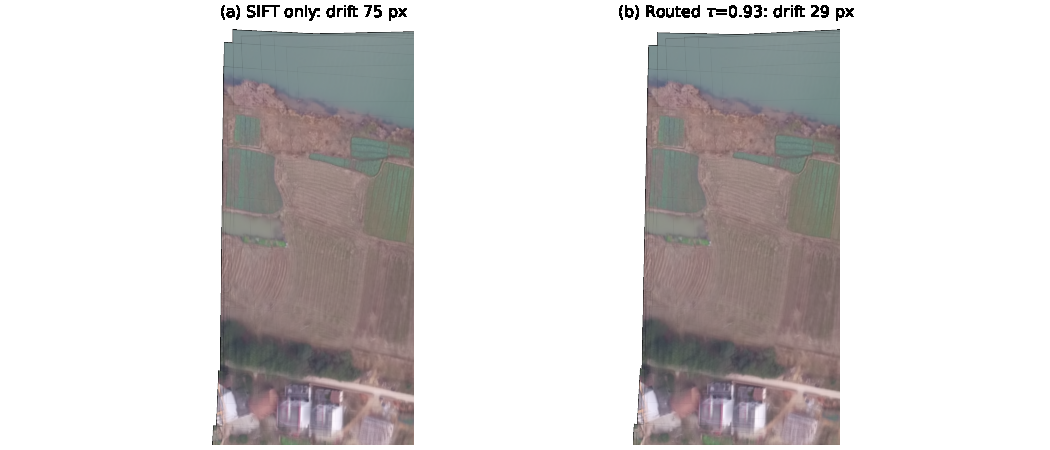
\includegraphics[width=\columnwidth]{figures/fig_mosaic_village.pdf}
\caption{Mosaics of the \texttt{village} window (46 frames, forward flight), rebuilt
from the stored homographies: (a) SIFT only, (b) routed at $\tau_{\mathrm{ncc}}{=}0.93$.
The strip silhouette is the warped frame boundary; the difference in drift
(75.3\,px vs.\ 28.5\,px) is measured, not read off the picture.}
\label{fig:mosaic_village}
\end{figure}

\begin{figure}[t]
\centering
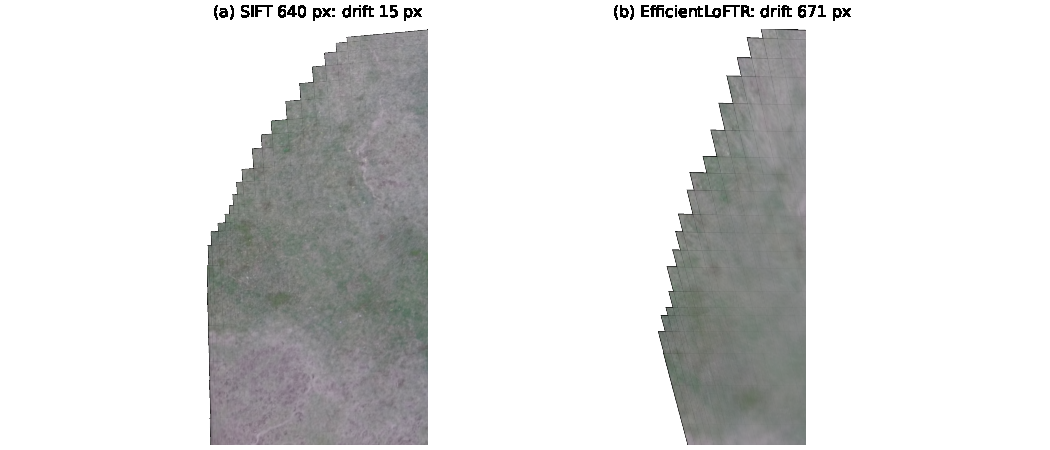
\includegraphics[width=\columnwidth]{figures/fig_mosaic_grass.pdf}
\caption{Same 46 frames of \texttt{grass}, two matchers, no recovery:
(a) SIFT at 640\,px, (b) Efficient LoFTR. The staircase shear on the right is
the accumulated 671.3\,px disagreement with the reference chain, on terrain
where the learned matcher reports dense, low-residual (but wrong) matches.}
\label{fig:mosaic_grass}
\end{figure}

\begin{table}[t]
\caption{RQ2, \texttt{village} window (45 steps). ``Strong'' = steps sent to
SuperPoint+LightGlue; time is matcher-stage time only.}\label{tab:rq2}
\centering\footnotesize
\setlength{\tabcolsep}{3pt}
\begin{tabular}{lcccc}
\toprule
Policy & Strong & Time (s) & $e_i$ mean (px) & Drift (px) \\
\midrule
SIFT only            & 0/45 & 3.2  & 2.51 & 75.3 \\
SP+LG only           & 45/45 & 60.4 & 2.67 & 82.4 \\
Routed $\tau{=}0.93$ & 7/45 & 13.3 & 2.42 & \textbf{28.5} \\
Routed + full-res    & 7/45 & 73.6 & \textbf{1.95} & 35.8 \\
\bottomrule
\end{tabular}
\end{table}

\begin{figure}[t]
\centering
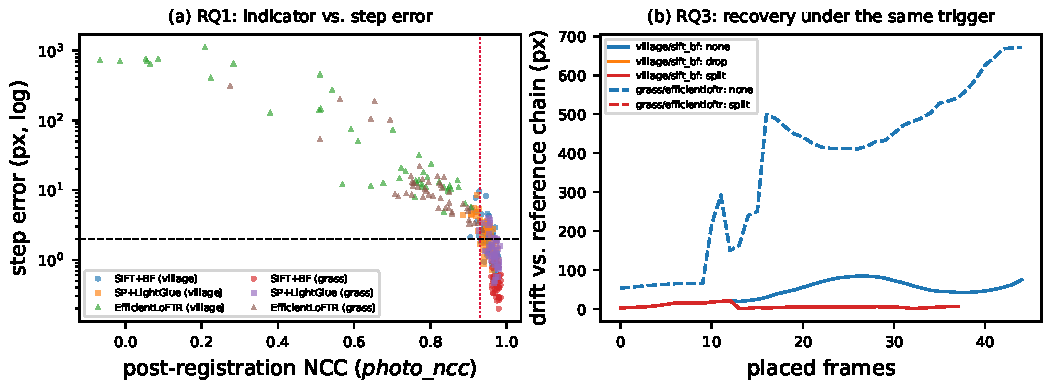
\includegraphics[width=\columnwidth]{figures/fig_rq1_rq3.pdf}
\caption{(a) Step error against the post-registration NCC indicator on both
windows and all three matchers; dashed line = 2\,px bad/good boundary, dotted
line = the selected trigger. (b) Drift against the reference chain for RQ3
policies under the same trigger. Split resets the coordinate frame at each
fragment, so its curve is piecewise, not a single chain.}
\label{fig:rq1rq3}
\end{figure}

\begin{figure}[t]
\centering
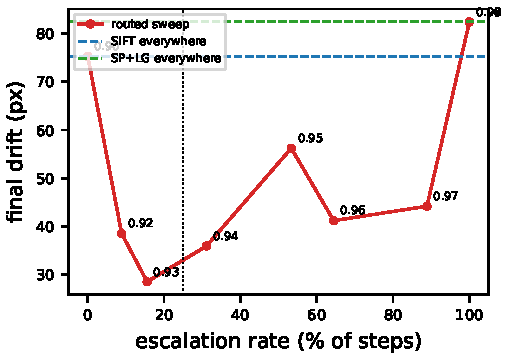
\includegraphics[width=0.62\columnwidth]{figures/fig_tau.pdf}
\caption{RQ2 threshold sweep on \texttt{village}: escalation rate against
final drift. Horizontal lines are the two fixed policies; the dotted line is
the 25\% escalation budget. Drift is non-monotone in $\tau$, so the operating
point is chosen by budget, not by ``higher threshold = safer''.}
\label{fig:tau}
\end{figure}

\subsection{RQ3: recovery under one trigger}
Table~\ref{tab:rq3} reports both windows. On village (7 initial triggers),
\emph{split} places all 46 frames across 8 submosaics, chaining 38 of 45 steps
with a maximum internal drift of 21.7\,px; \emph{drop} and \emph{anchor} keep
only 14/46 frames (13 chained steps, the same 21.7\,px ceiling), because dropping one frame enlarges the overlap gap
of the next pair and triggers the guard again (7 initial triggers cascade to
32). \emph{anchor} performs identically to \emph{drop} here: with every
remaining candidate either already-rejected or unplaced, no safe anchor frame
existed. Fig.~\ref{fig:mosaic_split} shows what the split policy actually
produces.

On grass with Efficient LoFTR, 44 of 45 steps are flagged. \emph{drop} and
\emph{anchor} place a single frame (the map does not survive); \emph{split}
keeps all 46 frames but degenerates into 45 one-frame fragments with a single
chained step. Low drift there is an artefact of that fragmentation, not
evidence of a recovered map.

\begin{figure}[t]
\centering
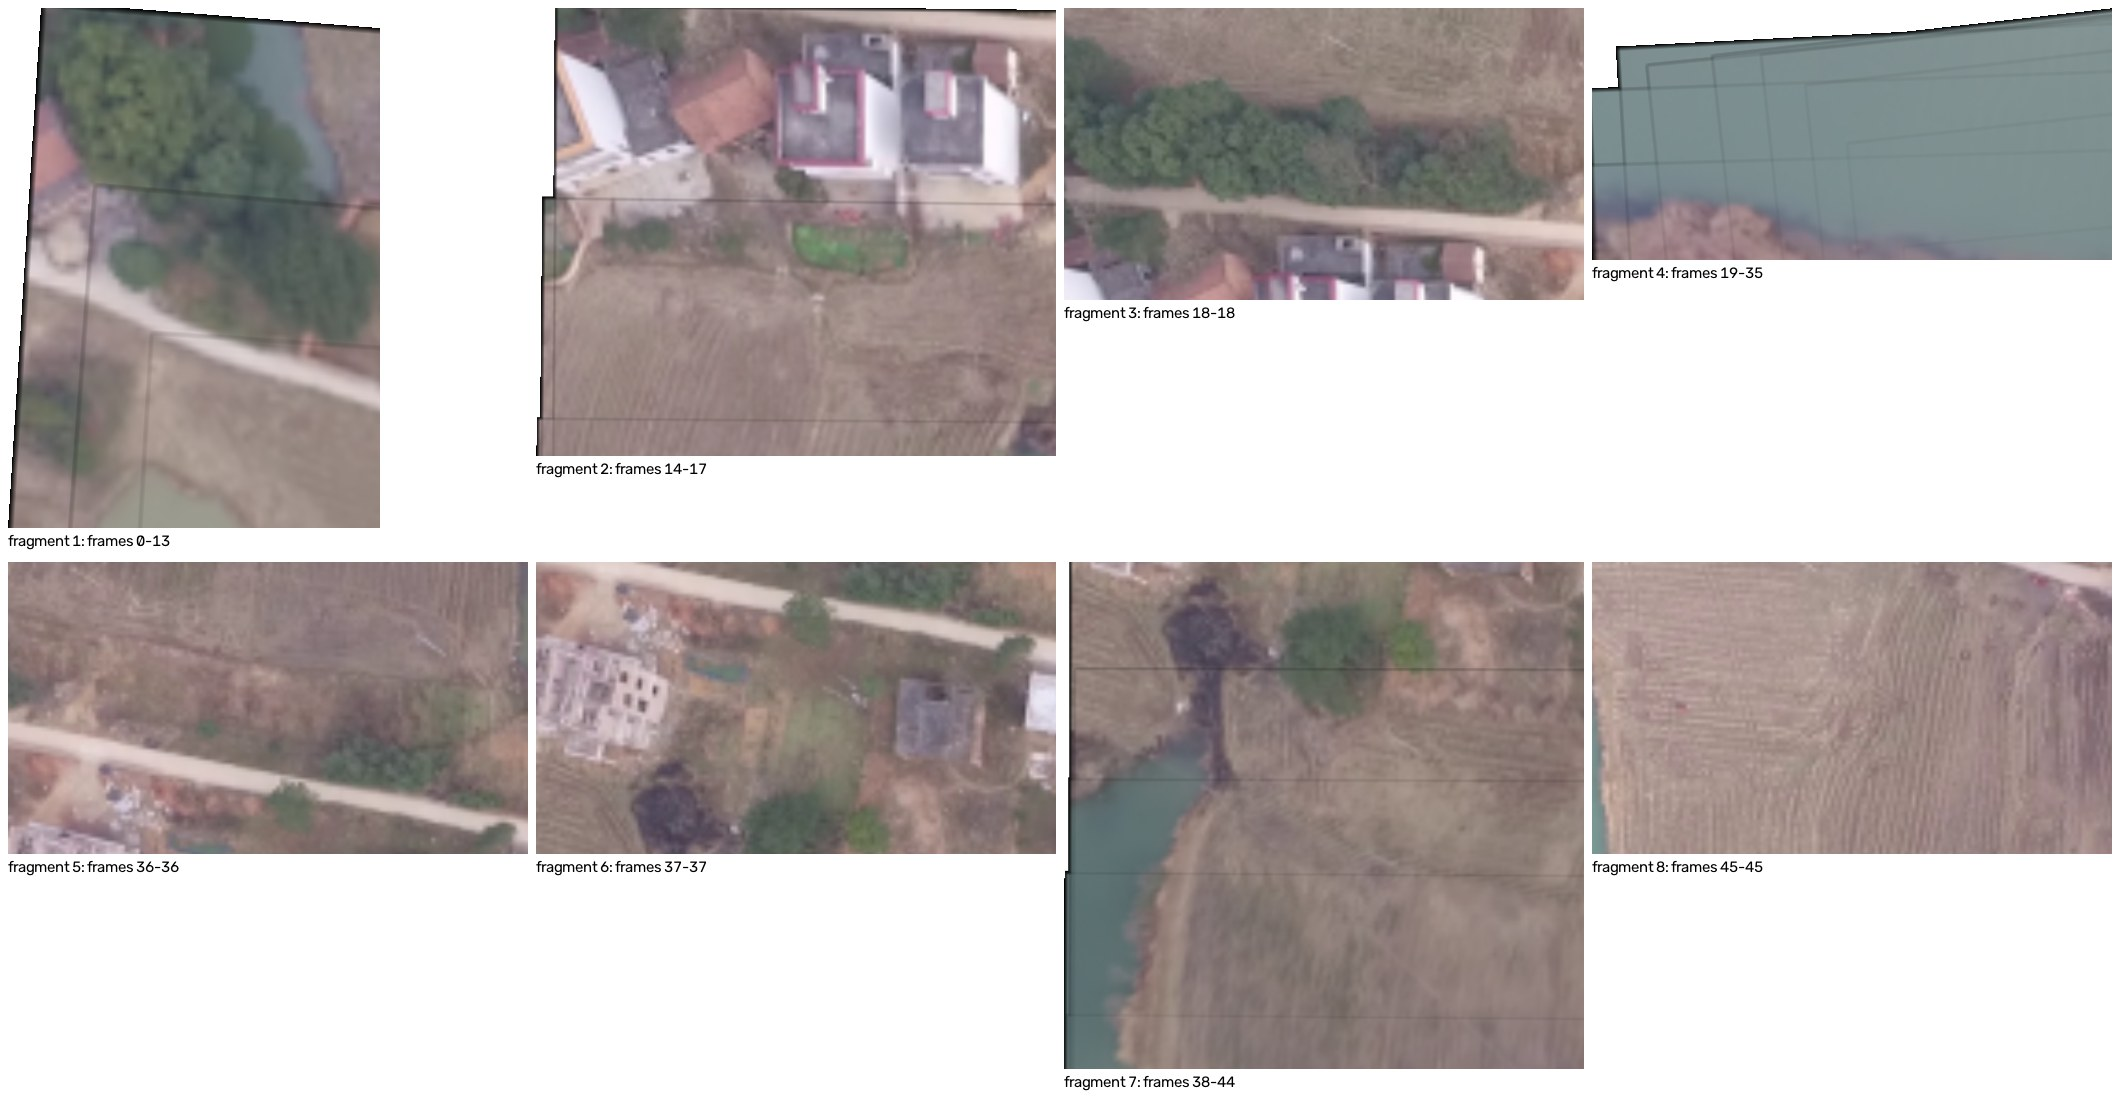
\includegraphics[width=\columnwidth]{figures/mosaic_village_split.jpg}
\caption{Split policy on \texttt{village}: the same 46 frames, cut at the 7 flagged
steps into 8 fragments, each in its own coordinate frame. All frames survive,
but the downstream consumer receives 8 disconnected surfaces, four of which
(fragments 3, 5, 6 and 8) are single frames.}
\label{fig:mosaic_split}
\end{figure}

\begin{table}[t]
\caption{RQ3: recovery policies at the RQ2-selected trigger
(village $\tau{=}0.93$, grass $\tau{=}0.96$). Drift is the maximum internal
drift within a chain; split resets the frame per fragment, and n/a means no
frame was placed, so there is nothing to measure.}\label{tab:rq3}
\centering\footnotesize
\setlength{\tabcolsep}{3pt}
\begin{tabular}{llccr}
\toprule
Window / matcher & Policy & Frames kept & Fragments & Drift (px) \\
\midrule
village / SIFT & none   & 46/46 & 1  & 84.6 \\
village / SIFT & drop   & 14/46 & 1  & 21.7 \\
village / SIFT & anchor & 14/46 & 1  & 21.7 \\
village / SIFT & split  & 46/46 & 8  & 21.7 \\
grass / ELoFTR & none   & 46/46 & 1  & 671.3 \\
grass / ELoFTR & drop   & 1/46  & 1  & n/a \\
grass / ELoFTR & split  & 46/46 & 45 & 2.7 \\
\bottomrule
\end{tabular}
\end{table}

\section{Discussion}\label{sec:disc}
\textbf{Cheap does not mean informative.} Match and inlier counts, the
indicators named in most acceptance heuristics, carried no usable signal at
step level in our window, and the data inverted their declared direction
(fewer matches is suspicious): steps with many matches can still be placed
consistently with a wrong geometry. Indicators computed \emph{after}
registration (photometric agreement, internal residual, projected overlap)
carry the signal. The practical cost is that they cannot be evaluated before
matching, so our trigger is a post-hoc guard applied to the cheap matcher's
output, not a pre-matching predictor.

\textbf{Spending more compute is not monotone in quality.} Always-learned
ended worse than SIFT-only on village, and per-step accuracy improved by
escalating at full resolution did not translate into lower chain drift. The
plausible mechanism is that the accumulated map is a product of the whole
chain, not of the average step: a locally better-conditioned $H_i$ changes
which frame geometries are compensated later. We treat this as a hypothesis;
testing it requires varying the escalation set independently of the trigger.

\textbf{Threshold selection is the hard part.} Fig.~\ref{fig:tau} shows the
sweep is U-shaped: 15.6\% escalation is the best point measured, while
escalating half the steps (53\%) is worse than escalating none. A budget rule
(``largest $\tau$ such that escalation stays below 25\%'') produced 0.93/0.96
on the two windows, but a rule that assumes monotonicity over a range where
the metric is non-monotone is only as good as the windows it was fitted on.

\textbf{Recovery trade-off is frames vs.\ connectivity.} Split preserves the
frame inventory but fragments the map (8 pieces for 46 frames, 45 pieces in
the degenerate case); drop/anchor preserve continuity of the surviving chain
but cascade under a conservative trigger, losing 70\% of frames here. Which is
preferable depends on whether the downstream use needs coverage or a single
geometric surface; a question our numbers cannot settle, and one reason the
mosaic images for each policy should be inspected before drawing conclusions.

\section{Limitations}
\textbf{Error proxy.} All errors are disagreement with a full-resolution SIFT
reference chain, which itself accumulates error; nothing here is validated
against field geometry (no GCP/orthophoto comparison in this draft), so
absolute drift values should not be read as georeferencing accuracy.

\textbf{Sample.} Two of the 14 public NPU Drone-Map packages, two windows
chosen \emph{because} they are hard. Base rates of bad steps (21/45, 6/38,
45/45) are properties of that selection and must not be read as deployment
expectations. There is no held-out sequence yet, and the trigger and budget
have not been re-tested on the remaining packages.

\textbf{Selection and multiplicity.} Indicators, direction, the 2\,px
boundary and $\tau$ were all chosen while looking at these windows; the
direction was fixed in advance to remove the most obvious leak, but the
results remain exploratory rather than confirmatory. The 45 steps are also
temporally dependent, not 45 independent samples.

\textbf{Cost accounting.} The time column measures the matcher stage only.
RANSAC, warping, the photometric checks and the risk decision are excluded, so
this draft supports no end-to-end latency claim; the true routing overhead is
higher than 13.3\,s and the true always-learned overhead also includes its
own post-processing.

\textbf{Integration.} RQ3 runs a fixed matcher per window and does not use the
routes produced in RQ2; an end-to-end ``cheap $\to$ escalate $\to$ recover''
run, its mosaic outputs, and per-fragment connectivity measures are still
missing. All timings come from one CPU-only machine.

\section{Conclusion}
On an incremental-homography UAV pipeline, the cheap indicators that predict
useful step-level risk are not the point counts that acceptance heuristics
usually use but post-registration evidence; a classical-first router with a
budget-selected trigger cut final drift by 62\% at 4.1$\times$ the cheap
matcher's time while calling the learned matcher everywhere was slower and
worse; and under one shared trigger, frame-preserving submosaic splitting kept
all frames where drop/anchor cascaded to 14/46. Next steps, in order: re-run
the same notebook unchanged on held-out packages, integrate routing with
recovery into one end-to-end run with full-pipeline timing, validate against
field geometry, and inspect the per-policy mosaics.

\begin{thebibliography}{00}
\bibitem{lowe2004} D. G. Lowe, ``Distinctive image features from scale-invariant keypoints,'' \emph{Int. J. Comput. Vis.}, vol. 60, no. 2, pp. 91--110, 2004.
\bibitem{rublee2011} E. Rublee, V. Rabaud, K. Konolige, and G. Bradski, ``ORB: An efficient alternative to SIFT or SURF,'' in \emph{Proc. IEEE Int. Conf. Comput. Vis. (ICCV)}, 2011, pp. 2564--2571.
\bibitem{fischler1981} M. A. Fischler and R. C. Bolles, ``Random sample consensus: A paradigm for model fitting with applications to image analysis and automated cartography,'' \emph{Commun. ACM}, vol. 24, no. 6, pp. 381--395, 1981.
\bibitem{detone2018} D. DeTone, T. Malisiewicz, and A. Rabinovich, ``SuperPoint: Self-supervised interest point detection and description,'' in \emph{Proc. IEEE/CVF Conf. Comput. Vis. Pattern Recognit. Workshops (CVPRW)}, 2018, pp. 224--236.
\bibitem{lindenberger2023} P. Lindenberger, P.-E. Sarlin, and M. Pollefeys, ``LightGlue: Local feature matching at light speed,'' in \emph{Proc. IEEE/CVF Int. Conf. Comput. Vis. (ICCV)}, 2023.
\bibitem{sun2021} J. Sun, Z. Shen, Y. Wang, H. Bao, and X. Zhou, ``LoFTR: Detector-free local feature matching with transformers,'' in \emph{Proc. IEEE/CVF Conf. Comput. Vis. Pattern Recognit. (CVPR)}, 2021, pp. 8922--8931.
\bibitem{wang2024} Q. Wang \emph{et al.}, ``Efficient LoFTR: Semi-dense local feature matching with sparse-like speed,'' in \emph{Proc. IEEE/CVF Conf. Comput. Vis. Pattern Recognit. (CVPR)}, 2024.
\bibitem{potlapalli2024} P. Potlapalli, P. Lindenberger, and M. Pollefeys, ``XFeat: Accelerated features for lightweight image matching,'' in \emph{Proc. IEEE/CVF Conf. Comput. Vis. Pattern Recognit. (CVPR)}, 2024.
\bibitem{hwang2026} D. Hwang \emph{et al.}, ``Real-time 2D orthomosaic mapping using CPU-based incremental homography matrix estimation with UAV video,'' \emph{Appl. Sci.}, vol. 16, no. 4, p. 2133, 2026.
\bibitem{li2023} X. Li \emph{et al.}, ``A real-time incremental video mosaic framework for UAV remote sensing,'' \emph{Remote Sens.}, vol. 15, no. 8, p. 2127, 2023.
\bibitem{dronezaic} M. Kharismawati and D. Kazic, ``DroneZaic: A robust end-to-end pipeline for mosaicking freely flown aerial video of agricultural fields,'' \emph{Plant Phenome J.}, vol. 8, no. 1, p. e70033, 2025.
\bibitem{chen2022} J. Chen \emph{et al.}, ``UAV video stitching based on optimal seamline and half-projective warp,'' \emph{Remote Sens.}, vol. 14, no. 5, p. 1068, 2022.
\bibitem{kim2025} J. Kim and S. Kim, ``Robust UAV image mosaicking using SIFT and LightGlue,'' \emph{Int. Arch. Photogramm. Remote Sens. Spatial Inf. Sci.}, vol. XLVIII-2-W11-2025, pp. 169--173, 2025.
\bibitem{gaisbauer2025} S. Gaisbauer, P. Gyawali, Q. Zhang, O. Wysocki, and B. Jutzi, ``To glue or not to glue? Classical vs learned image matching for mobile mapping cameras to textured semantic 3D building models,'' \emph{ISPRS Ann. Photogramm. Remote Sens. Spatial Inf. Sci.}, vol. X-1/W2-2025, 2025.
\bibitem{zaffar2024} M. Zaffar \emph{et al.}, ``On the estimation of image-matching uncertainty in visual place recognition,'' in \emph{Proc. IEEE/CVF Conf. Comput. Vis. Pattern Recognit. (CVPR)}, 2024.
\bibitem{sferrazza2024} C. Sferrazza \emph{et al.}, ``To match or not to match: Evaluating keypoint matching confidence for visual place recognition,'' in \emph{Proc. CVPRW}, 2024.
\bibitem{barath2023} D. Barath \emph{et al.}, ``A large-scale homography benchmark,'' in \emph{Proc. IEEE/CVF Conf. Comput. Vis. Pattern Recognit. (CVPR)}, 2023.
\bibitem{yuan2024} H. Yuan, D. Peng, and M. Dong, ``Comparative analysis of color space transformations on feature-based image registration,'' \emph{J. Imaging}, vol. 10, no. 5, p. 105, 2024.
\bibitem{ivashechkin2021} M. Ivashechkin, D. Barath, and J. Matas, ``VSAC: Efficient and accurate estimator for H and F,'' in \emph{Proc. IEEE/CVF Int. Conf. Comput. Vis. (ICCV)}, 2021.
\bibitem{uasthn} J. Xiao and G. Loianno, ``UASTHN: Uncertainty-aware deep homography estimation for UAV satellite--thermal geo-localization,'' arXiv:2502.01035, 2025.
\bibitem{dalglue} H. Zhang, H. He, Y. Zhou, and F. Lei, ``Efficient image matching for UAV visual navigation via DALGlue,'' \emph{Sci. Rep.}, vol. 15, p. 37684, 2025.
\bibitem{map2dfusion} S. Bu, Y. Zhao, G. Wan, and Z. Liu, ``Map2DFusion: Real-time incremental UAV image mosaicing based on monocular SLAM,'' in \emph{Proc. IEEE/RSJ Int. Conf. Intell. Robots Syst. (IROS)}, 2016.
\end{thebibliography}

\end{document}
